\section{Simulazione modello lineare}
Riprendendo l'equazione (\ref{equazionemoto}), l'analisi del sistema può essere schematizzata in forma ridotta attraverso l'equazione 
\begin{equation}
    M\ddot y+\bar c\dot y+\bar k y=F(t)
    \label{equazionemodello}
\end{equation}
dove $F(t)=me\omega^2\sin(\omega t)$ rappresenta una forzante periodica sul sistema, mentre  $\bar c=1.5 c$ e $\bar k=1.5 k$ rappresentano rispettivamente i coefficienti di smorzatore e molla equivalente del sistema.

Da questa espressione si può derivare graficamente il modello vibrazionale equivalente della lavatrice oggetto di studio (Figura \ref{ModelloVibrazionale}). 
\begin{figure}[h]
    \centering
    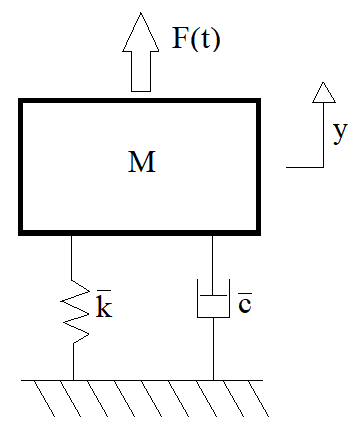
\includegraphics[scale=0.7]{Immagini/Massa-molla-smorzatore.png}
    \caption{Modello vibrazionale semplificato.}
    \label{ModelloVibrazionale}
\end{figure}

Si è voluta arricchire la trattazione implementando in ambiente di calcolo il modello analitico-lineare precedentemente ottenuto. \textit{Simulink} e \textit{Simscape} sono i software utilizzati per tale scopo.
\subsection{Simulink}
 Il  software  \textit{Simulink}  è  un  applicativo  situato all'interno  di \textit{Matlab} e ne costituisce una potente e intuitiva interfaccia grafica. Mediante \textit{Simulink} è possibile “programmare” l'esecuzione di calcoli in maniera molto più rapida ed error-free rispetto alla scrittura dei lunghi e complessi m-files. 
 
 Gli  strumenti visuali disponibili in ambiente \textit{Simulink} permettono di  simulare  dei sistemi  anche  molto  complessi attraverso il tracciamento, su  un  foglio  di  lavoro  elettronico, di  uno  schema  a  blocchi  rappresentativo del sistema in esame.
 
 \paragraph{Modello Simulink} Per modellare un sistema coerente con la trattazione fin qui svolta, è stata rielaborata l'equazione (\ref{equazionemodello}) in modo da ottenere al primo membro solo il termine contenente la massa $M\ddot y=F(t)-\bar c \dot y-\bar k y$.
 
 Il modello ottenuto è visibile in Figura \ref{ModelloSimulink}.
 \begin{figure}[ht]
    \centering
    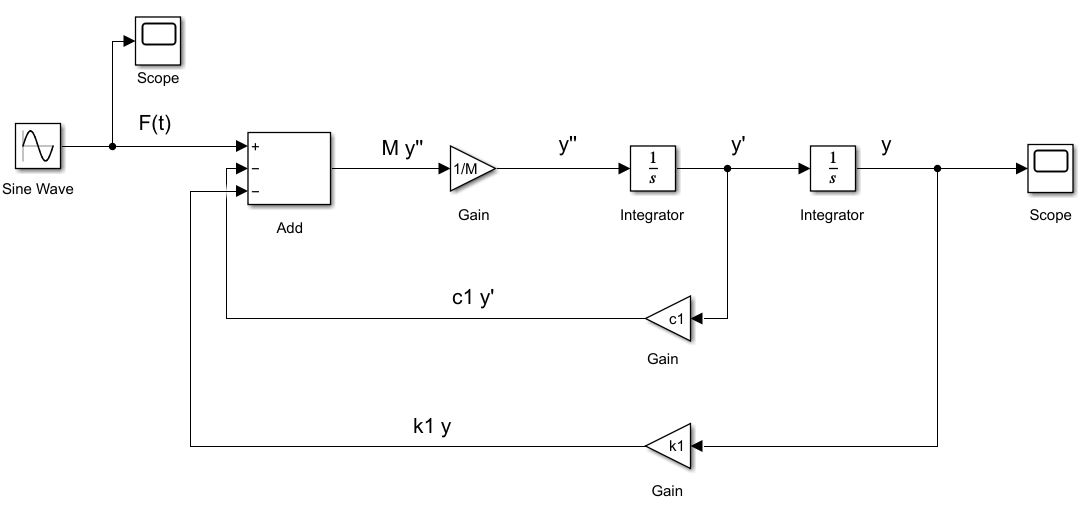
\includegraphics[width=\textwidth]{Immagini/Modello simulink.JPG}
    \caption{Modello Simulink.}
    \label{ModelloSimulink}
\end{figure}

Si è creato una forzante sinusoidale attraverso il blocco \textit{Sine Wave}, la cui ampiezza è stata calcolata attraverso la variabile $A=m*e*(\omega^2)$. Successivamente si è aggiunto un blocco \textit{Add} che sommasse le forze di molla equivalente, smorzatore equivalente e forzante, in modo tale da ottenere in uscita il termine in massa $M\ddot y$. 

A questo punto, un blocco \textit{Gain}, ha permesso di moltiplicare il termine in uscita da \textit{Add} della quantità $\frac{1}{M}$, in modo da ottenere l'accelerazione dell'asse del cestello. Due blocchi \textit{Integrator} posti in serie hanno premesso prima di ricavare la velocità e poi la posizione del cestello. Tali grandezze sono state moltiplicate attraverso blocchi \textit{Gain} delle quantità rappresentative della molla e smorzatore equivalente, per ottenere le forze da aggiungere al blocco \textit{Add} di cui si è parlato precedentemente, creando una sorta di sistema in retroazione. 

Infine, il blocco \textit{Scope} ha permesso di ottenere un grafico dello spostamento lungo il sistema di riferimento dell'asse del cestello nel tempo.
\paragraph{Script di caricamento variabili} Per aggiungere maggiore generalità al modello, si è pensato di stilare uno script \textit{Matlab} in cui inserendo le specifiche tecniche della lavatrice e del peso dei panni bagnati da lavare, la simulazione restituisse la corrispondente ampiezza di spostamento dell'asse del cestello in funzione del tempo. 

I dati sono stati presi in input a seguito di una richiesta a display del programma di tipo:
\begin{lstlisting}[frame=trBL]
prompt = 'Inserire massa in kg del cestello: ';
prompt1 = 'Inserire massa in kg dei panni da lavare: ';
prompt2 = 'Inserire coefficienti elastici delle molle in
           N/m: ';
prompt3 = 'Inserire coefficienti di smorzamento viscoso in
           Ns/m: ';
prompt4 = 'Inserire raggio del cestello in m: ';
prompt5 = 'Inserire giri al minuto della centrifuga';
\end{lstlisting}
Ai dati inseriti sono state collegate le variabili corrispondenti alle caratteristiche della lavatrice:
\begin{lstlisting}[frame=trBL]
M = input(prompt);
m_asciutta = input(prompt1);
k = input(prompt2);
c = input(prompt3);
e = input(prompt4);
rpm = input(prompt5);
\end{lstlisting}
Per adattare i dati in input al modello studiato sono state svolte alcune operazioni elementari:
\begin{itemize}
    \item considerata la massa dei panni da bagnata (m)
    \item considerato coefficiente elastico della molla equivalente (k1)
    \item considerato coefficiente di smorzamento viscoso equivalente (c1)
    \item convertito in radianti al secondo i giri al minuto della centrifuga (omega)
    \item calcolato ampiezza della forzante sinusoidale (A) 
\end{itemize}

\begin{lstlisting}[frame=trBL]
m = 2*m_asciutta;
k1 = 1.5*k;
c1 = 1.5*c;
omega = 0.14072*rpm;
A = m*e*(omega^2);
\end{lstlisting}
La simulazione si serve quindi delle seguenti variabili:
\begin{itemize}
    \item M
    \item m
    \item k1
    \item c1
    \item e
    \item omega
    \item A.
\end{itemize}

Come risultato dello studio del modello, si è provato a simulare attraverso parametri realistici il comportamento vibrazionale della lavatrice. Inserendo i seguenti dati:
\begin{itemize}
    \item M = 30 [kg];
    \item m\_asciutta = 5 [kg];
    \item k = 5000 [N/m];
    \item c = 350 [Ns/m];
    \item e = 0.25 [m];
    \item rpm = 450 [rpm];
\end{itemize}
si ottiene uno spostamento dell'asse del cestello nel tempo lungo il rifermento, come mostrato in Figura \ref{PrimoPlot}. 
\begin{figure}[h]
    \centering
    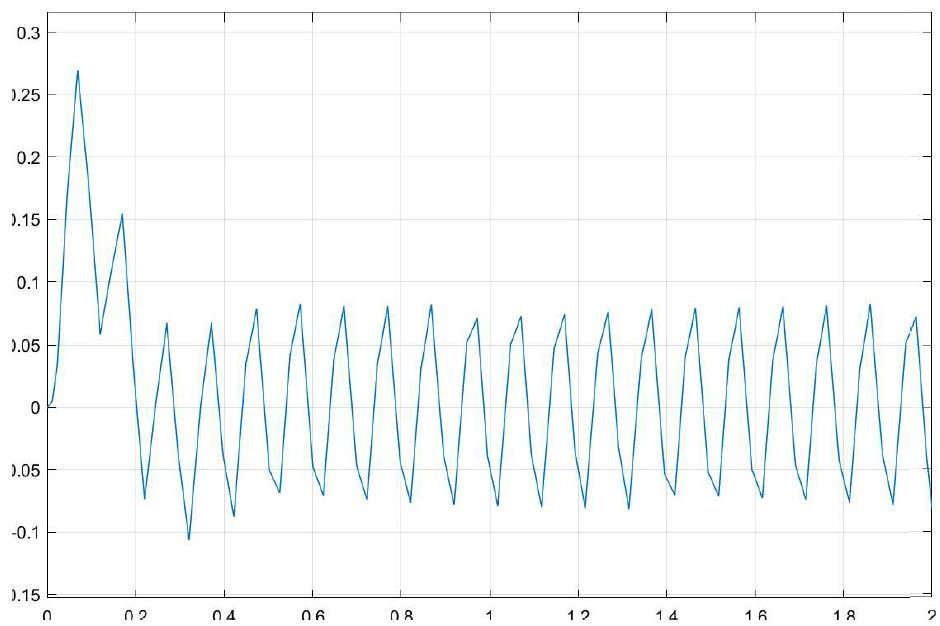
\includegraphics[scale=0.5]{Immagini/PrimoPlot.JPG}
    \caption{Oscillazione asse cestello lungo il riferimento.}
    \label{PrimoPlot}
\end{figure}
A seguito di un transitorio iniziale, l'oscillazione si stabilizza secondo un andamento armonico.
Attraverso l'equazione (\ref{Ampiezza}) è stato calcolato analiticamente uno spostamento $Y=0.085$ [m].

L'architettura della simulazione è tale da consentire di variare i parametri in ingresso per apprezzarne l'effetto sull'uscita, attraverso un riscontro grafico.
\\\\
A titolo di esempio si è voluta modificare la configurazione del sistema aumentando i coefficienti di smorzamento viscoso e i coefficienti elastici:
\begin{itemize}
    \item k = 10000 [N/m]; $\to$ k1=15000 [N/m];
    \item c = 1000 [Ns/m]; $\to$ c1=1500 [Ns/m];
\end{itemize}
il risultato è apprezzabile in Figura \ref{SecondoPlot}. Anche in questo caso,  attraverso l'equazione (\ref{Ampiezza}), è stato calcolato analiticamente uno spostamento $Y=0.07$ [m].
\begin{figure}[h]
    \centering
    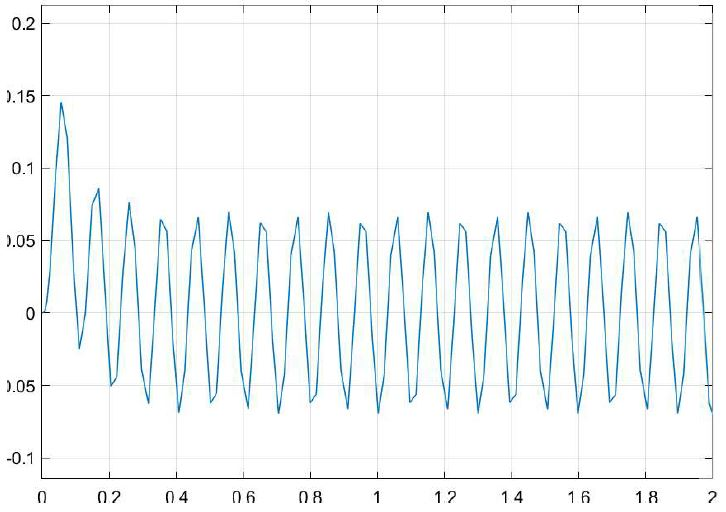
\includegraphics[scale=0.6]{Immagini/SecondoPlot.JPG}
    \caption{Oscillazione asse cestello lungo il riferimento.}
    \label{SecondoPlot}
\end{figure}
\subsection{Simscape}
Con \textit{Simscape} si possono creare rapidamente modelli di sistemi fisici all’interno dell’ambiente \textit{Simulink}. \textit{Simscape} consente di costruire modelli di componenti meccanici basati su collegamenti che si integrano direttamente con diagrammi a blocchi e altri paradigmi di modellazione. 

Il modello fisico del sistema realizzato attraverso questo software vede blocchi corrispondenti direttamente ai componenti fisici del sistema. Questa caratteristica consente di rendere più intuitiva la modellazione a scapito della flessibilità di analisi. Più in dettaglio, se nel modello realizzato con \textit{Simulink} le variabili rappresentative delle caratteristiche della lavatrice potevano essere cambiate direttamente utilizzando lo script di \textit{Matlab}, con \textit{Simscape} bisogna intervenire direttamente sul modello, inserendo manualmente il valore dei coefficienti equivalenti di molla e smorzatore. 
\paragraph{Modello Simscape} Il software in questione ha consentito lo sviluppo di un modello di calcolo del tutto simile a quello rappresentato in Figura \ref{ModelloVibrazionale}. 
\begin{figure}[ht]
    \centering
    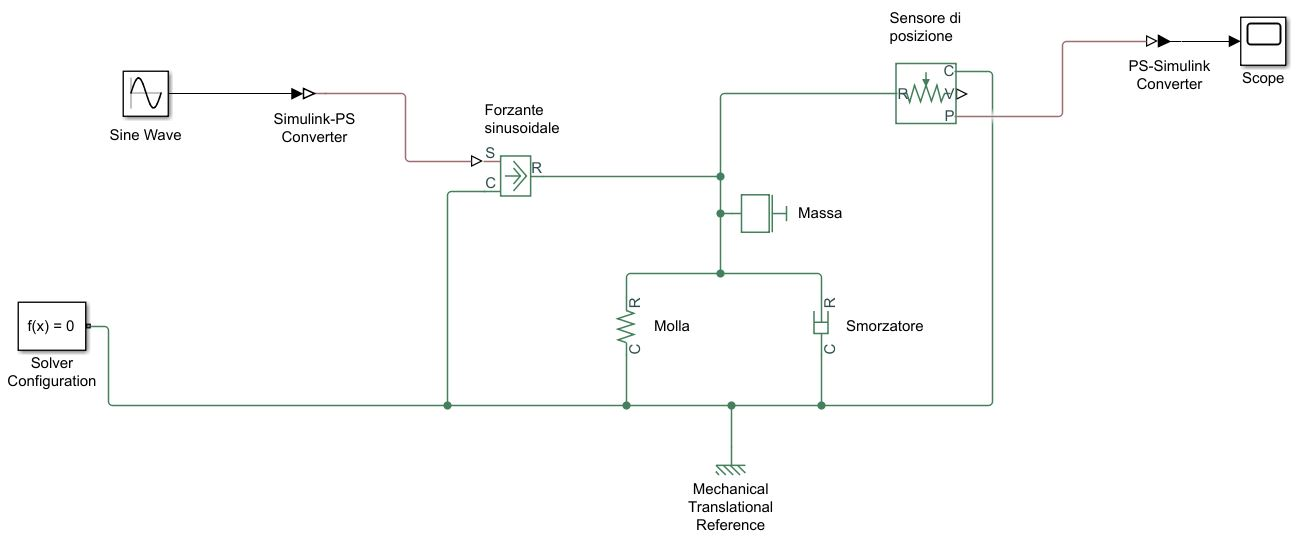
\includegraphics[width=\textwidth]{Immagini/ModelloSimscape.JPG}
    \caption{Modello Simscape.}
    \label{ModelloSimscape}
\end{figure}

In ambiente \textit{Simscape} è importante identificare il riferimento e il modo in cui i vari blocchi vengono collegati tra loro. In questo caso si è partiti dal riferimento a terra (\textit{Mechanical Traslational Reference}) per proseguire con l'inserimento in parallelo dei blocchi di molla e smorzatore. 

Per la risoluzione del modello è necessario implementare un blocco risolutore chiamato \textit{Solver Configuration} che può essere collegato ovunque all'interno del modello, per chiarezza è stato collocato a riferimento. 

La massa rappresentativa del cestello rotante è collegata a molla e smorzatore equivalenti. Questi ultimi tre blocchi rappresentano i componenti fisici del modello oggetto di studio. 

Alla massa è stata inoltre collegata una forzante del tutto identica a quella utilizzata nel modello \textit{Simulink}. La traduzione del segnale generato dal blocco \textit{Sine Wave}, ad opera dell'operatore \textit{Simulink-PS Converter}, ha consentito attraverso l'utilizzo del blocco \textit{Ideal Force Source} di generare una forza a partire dalle caratteristiche del segnale in ingresso. 

Infine, per rilevare lo spostamento della massa del cestello nel tempo a causa della forzante, è stato inserito un blocco rappresentativo di un sensore di posizione. In uscita a quest'ultimo, il \textit{PS-Simulink Converter} ha consentito una traduzione del segnale in ambiente \textit{Simulink}, rendendo leggibile da un blocco \textit{Scope} e consentendone la visualizzazione grafica dello spostamento nel tempo. 

Quanto è stato svolto per la simulazione con modello \textit{Simulink} è replicato in ambiente \textit{Simscape}. Infatti, le variabili adottate attraverso lo script interattivo sono rimaste invariate in modo da poter comparare i due modelli. Come precedentemente spiegato, si sono dovuti inserire manualmente i coefficienti equivalenti comparsi nel \textit{Workspace}. 

Il risultato dello spostamento dell'asse del cestello nel tempo è visibile in Figura \ref{PrimoPlotSimscape}.
\begin{figure}[h]
    \centering
    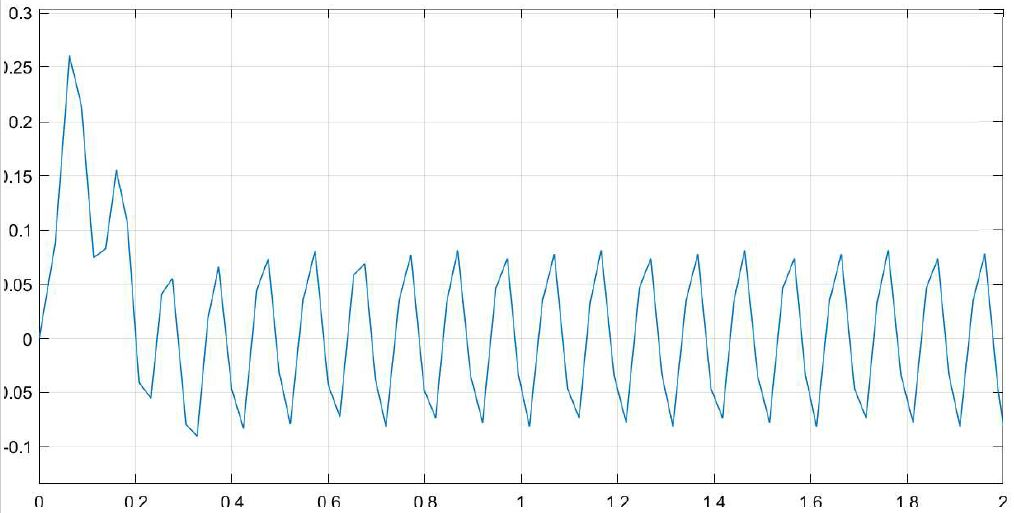
\includegraphics[scale=0.5]{Immagini/PrimoPlotSimScape.JPG}
    \caption{Oscillazione asse cestello lungo il riferimento.}
    \label{PrimoPlotSimscape}
\end{figure}

Coerentemente con quanto elaborato precedentemente, si è voluto simulare un secondo modello variando unicamente i coefficienti equivalenti di molla e smorzatore, con valori analoghi a quelli di pagina 21 (k1= 15000 N/m; c1=1500 Ns/m).

Il risultato ottenuto è visibile in Figura \ref{SecondoPlotSimscape}.\\
\begin{figure}[h]
    \centering
    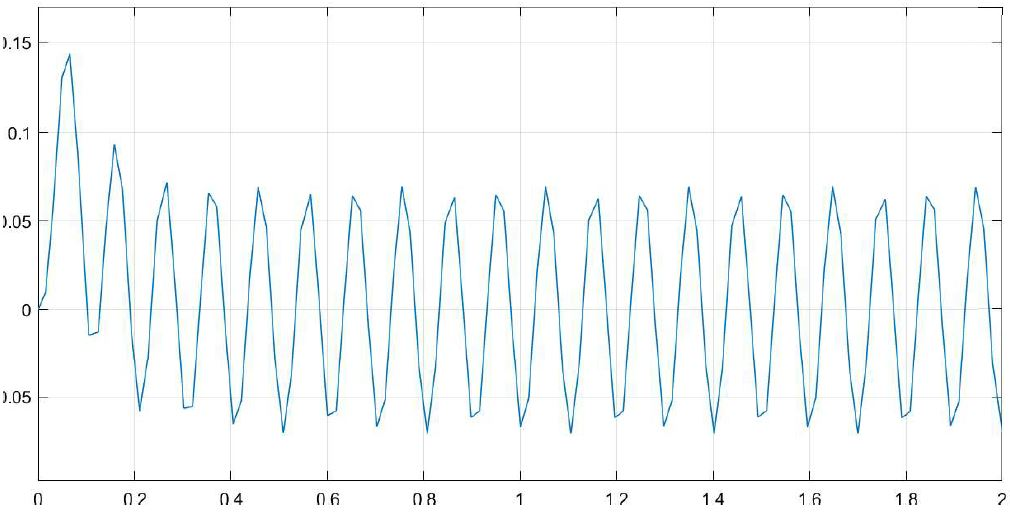
\includegraphics[scale=0.5]{Immagini/SecondoPlotSimScape.JPG}
    \caption{Oscillazione asse cestello lungo il riferimento.}
    \label{SecondoPlotSimscape}
\end{figure}

